%!TEX program = xelatex
%!TEX encoding = UTF-8 Unicode

\documentclass[10pt, twocolumn]{article}
\usepackage[top=1in, bottom=1in, left=1in, right=1in]{geometry}

% ----- ADDITIONAL PACKAGES -----
\usepackage{fontspec,xltxtra,xunicode}
\usepackage[usenames,dvipsnames]{color}
\usepackage[bookmarks, colorlinks, breaklinks, 
  pdfauthor={Yue Wu},
  pdfcreator={xelatex}
]{hyperref}
\usepackage{amsmath}
\usepackage{amsfonts}
\usepackage{paralist}

% ----- SETTINGS -----
\setcounter{secnumdepth}{0}
\linespread{1.15}
\setlength\parindent{0pt}
\setlength\parskip{1ex plus 0.2ex minus 0.1ex}
\setlength\emergencystretch{3em}
\hypersetup{linkcolor=blue, citecolor=blue, filecolor=black, urlcolor=MidnightBlue}

% ----- DOCUMENT -----
\begin{document}
\pagestyle{myheadings}
\markright{Yue Wu}

\section*{Basic Statistics}
\begin{itemize}
\item Conditional Prob: $P(A|B)=P(A\cap B)/P(B)$
\item Independent $\Longleftrightarrow P(A\cap B)=P(A)P(B)$
\begin{table}[h] \centering
\begin{tabular}{|c|c|c|} \hline
RV $X$    & Prob. $f(x)$     & CDF $F(x)$               \\ \hline
Disc(pmf) & $\sum_xf(x)=1$   & $\sum_{y\leq x}f(y)$     \\ \hline
Cont(pdf) & $\int_xf(x)dx=1$ & $\int_{-\infty}^xf(y)dy$ \\ \hline
\end{tabular}
\end{table}
\item $X$ is continuous RV $\Rightarrow F(X) \sim \text{Unif}(0,1)$ 
\item $E[(X-\mu)^n]$ is the $n$th \emph{central moment} of $X$
\item $M_X(t)\equiv E[e^{tX}]$: \emph{moment generating function}
\item Under certain technical conditions, 
\[ E[X^k]=\frac{d^k}{dt^k}M_X(t)|_{t=0},\ k=1,2,\dots \]
\item $Var[X]=E[X^2]-E^2[X]$
\item $E[aX+b]=aE[X]+b$, $V[aX+b]=a^2V[X]$
\item Joint CDF: $F(x,y)\equiv P(X\leq x, Y\leq y),\ \forall x,y$
\item Joint PDF: $f(x,y)\equiv \frac{\partial^2}{\partial x\partial y}F(x,y)$
\item Marginal CDF: $F_X(x)=\int F(x,y)dy$
\item \emph{Independent} $\Longleftrightarrow f(x,y)=f_X(x)f_Y(y) \Longleftrightarrow f(x,y)=a(x)b(y)$ and domains are independent % $\Longleftrightarrow f(y|x)=f_Y(y)$
\item Conditional PDF: $f(y|x)\equiv f(x,y)/f_X(x)$
\item $E[Y|X=x]=\int yf(y|x)dy$, $E[E(Y|X)]=E[Y]$
\item $E[XY]=\iint xyf(x,y)dxdy$
\item $Cov(X,Y)\equiv E[(X-EX)(Y-EY)]=E[XY]-E[X]E[Y]$, $Var(X)=Cov(X,X)$ \\
$Cov(aX,bY)=abCov(X,Y)$ \\
$Cov(X\pm Y,Z)=Cov(X,Z)\pm Cov(Y,Z)$
\item $Corr(X,Y)\equiv Cov(X,Y)/\sqrt{V(X)V(Y)}$ \\ 
$Corr(aX,bY)=Corr(X,Y)$
\item Independent $\Rightarrow Cov(X,Y)=0$
\item $Var(X\pm Y)=Var(X)+Var(Y)\pm 2Cov(X,Y)$
\end{itemize}

\section*{Probability Distributions}
\begin{itemize}
\item $X\sim \text{Bernoulli}(p)$:
\[ f(x) = \left\{ 
  \begin{array}{c l}
    p & \quad \text{if $x=1$}\\
    1-p & \quad \text{if $x=0$}
  \end{array} \right.\]
$E[X]=p$, $Var(X)=p(1-p)$
\item $X\sim \text{Binomial}(n,p)$: \\
(\# of successes in $n$ $\text{Bern}(p)$ trials)
\[ f(x)={n \choose x}p^x(1-p)^{n-x} \]
$E[X]=np$, $Var(X)=np(1-p)$
\item $X\sim \text{Geometric}(p)$: \\
(\# of $\text{Bern}(p)$ trials until a success occurs)
\[ f(x) = (1-p)^{x-1}p \]
$E[X]=1/p$, $Var(X)=(1-p)/p^2$
\item $X\sim \text{NegBin}(r,p)$: the sum of $r$ iid $\text{Geom}(p)$
\[ f(x)={x-1 \choose r-1}(1-p)^{x-r}p^r,\ x=r,r+1,\dots \]
$E(X)=r/p$, $Var(X)=r(1-p)/p^2$
\item $X\sim \text{Poisson}(\lambda)$: 
\[ f(x) = \frac{e^{-\lambda}\lambda ^x}{x!},\ x=0,1,\dots \]
$E[x]=\lambda=Var(X)$
\item $X\sim \text{Uniform}(a,b)$: 
\[ f(x)=\frac{1}{b-a},\ E[X]=\frac{a+b}{2},\ V(X)=\frac{(b-a)^2}{12} \]
\item $X\sim \text{Exponential}(\lambda)$: time between Poi events
\[ f(x)=\lambda e^{-\lambda x},\ F(x)=1-e^{-\lambda x}, \]
$E[X]=1/\lambda$, $Var(X)=1/\lambda^2$. And 
\[ P(X>s+t|X>s)=P(X>t) \]
\emph{memoryless property} $\Uparrow$
\item $X\sim \text{Erlang}(k, \lambda)$: the sum of $k$ $\text{Exp}(\lambda)$
\[ f(x)=\frac{\lambda^kx^{k-1}e^{-\lambda x}}{(k-1)!},\ for\ x,\lambda\geq0 \]
\[ F(x)=1-\sum_{n=0}^{k-1}\frac{e^{-\lambda x}(\lambda x)^n}{n!} \]
$E(X)=k/\lambda$, $Var(X)=k/\lambda^2$
\item $X\sim \text{Beta}(a,b)$: \\ 
\[ E(X)=\frac{a}{a+b},\ V(X)=\frac{ab}{(a+b)^2(a+b+1)} \]
\item $X\sim \text{Gamma}(\alpha,\lambda)$: 
\[ E[X]=\alpha/\lambda,\ Var(X)=\alpha/\lambda^2 \]
\item $X\sim \text{Triangular}(a,b,c)$: $E(X)=(a+b+c)/3$
\item $X\sim \text{Normal}(\mu,\sigma^2)$: 
\[ f(x) = \frac{1}{\sqrt{2\pi\sigma^2}}\text{exp}\left[-\frac{(x-\mu)^2}{2\sigma^2}\right],\ x\in\mathbb{R} \]
$E[X]=\mu$, $V[X]=\sigma^2$, $M_X(t)=exp[\mu t+\frac{1}{2}\sigma^2t^2]$
\item $X\sim \text{LogNormal}(\mu,\sigma^2)$:
\[ f(x) = \frac{1}{x\sqrt{2\pi\sigma^2}}\text{exp}\left[-\frac{(\ln x-\mu)^2}{2\sigma^2}\right],\ x\in\mathbb{R}^+ \]
$E[X]=e^{\mu+\sigma^2/2}$, $V[X]=(e^{\sigma^2}-1)e^{2\mu+\sigma^2}$
\item \emph{Law of Large Numbers} (special case): 
\[ X_1,\dots,X_n \text{ are iid Nor} \Rightarrow \bar{X}_n\sim \text{Nor}(\mu,\sigma^2/n) \]
\item \emph{Central Limit Theorem}: If $X_1,\dots,X_n\stackrel{iid}{\sim}f(x)$, 
\[ Z_n\equiv \frac{\bar{X}_n-\mu}{\sigma/\sqrt{n}}\stackrel{d}{\longrightarrow}\text{Nor}(0,1) \]
\item $100(1-\alpha)\%$ \emph{Confidence Intervals}: 
\[ \mu\in[\bar{X}_n-z_{\alpha/2}\sqrt{\frac{\sigma^2}{n}},\bar{X}_n+z_{\alpha/2}\sqrt{\frac{\sigma^2}{n}}] \text{ or}\]
\[ \mu\in[\bar{X}_n-t_{\alpha/2,n-1}\sqrt{\frac{S^2}{n}},\bar{X}_n+t_{\alpha/2,n-1}\sqrt{\frac{S^2}{n}}] \]
in which, $S^2=\frac{1}{n-1}\sum_{i=1}^n(X_i-\bar{X}_n)^2$
\end{itemize}

\section*{Simulations}
\begin{itemize}
\item Monte Carlo Integration: 
\[ \hat{I}_n=\frac{b-a}{n}\sum_{i=1}^nf[a+(b-a)U_i] \]
is an \emph{unbiased} estimator of $\int_a^bf(x)dx$.
\item Hand Simulation: \#, arrival time, start time, service time, departure time, waiting time
\end{itemize}

\section*{Random Variables}
\begin{itemize}
\item Generators We Don't Use: 
\begin{inparaenum}
  \item Random Devices: tough to repeat; 
  \item Random Number Tables: cumbersome and slow, not random; 
  \item Mid-Square Method: positive serial correlation, occasionally degenerates; and
  \item Fibonacci: small numbers follow small number, not possible to get $X_{i-1} \leq X_{i+1} \leq X_{i}$ or $X_{i} \leq X_{i+1} \leq X_{i-1}$.
\end{inparaenum}
\item \emph{Linear Congruential Generator}: 
\[ X_i=(\sum_{j=1}^qa_iX_{i-j})\,\text{mod}\,m \]
\item Generating \emph{pseudo-random numbers} from LCG: 
\[ X_i=16807X_{i-1}\text{mod}(2^{31}-1),\ i=1,2,\dots \]
Then set $R_i=X_i/(2^{31}-1)$.
\item \emph{Tausworthe Generator}:
\[ B_i = \left(\sum_{j=1}^qc_jB_{i-j}\right) \text{mod } 2 \]
Usual implementation: 
\[ B_i = (B_{i-r} + B_{i-q}) \text{ mod } 2 \quad (0<r<q) \]
\item \textbf{Theorem 1}: When $X_0$ is odd and $a=8k+3$ or $a=8k+5$ for some $k$, $X_i=aX_{i-1}\text{ mod }2^n$ ($n>3$) can have cycle length of at most $2^{n-2}$.
\item \textbf{Theorem 2}: $X_i=(aX_{i-1}+c)\text{ mod }m$ ($c>0$) has full cycle if 
\begin{inparaenum}
  \item $c$ and $m$ are relatively prime; 
  \item $a-1$ is a multiple of every prime which divides $m$; and 
  \item $a-1$ is a multiple of $4$ if $4$ divides $m$.
\end{inparaenum}
\item \textbf{Theorem 3}: $X_i=aX_{i-1}\text{ mod }m$ wirh prime $m$ has full period $(m-1)$ $\Leftrightarrow$ $m$ divides $a^{m-1}-1$ and $m$ doesn't divide $a^i-1$ for all $i<m-1$.
\item \textbf{Theorem 4}: The $k$-tuples from multiplicative generators lie on parallel hyperplanes in $[0,1]^k$.
\item \emph{Runs Tests ``Up and Down''}: % \\ (a series of similar observations)
\[ |Z_0| = \frac{|A-E[A]|}{\sqrt{\text{Var}(A)}} \leq z_{\alpha/2} \]
$A \approx \text{Nor}((2n-1)/3, (16n-29)/90)$ is the \# of runs ``up and down'' out of $n$ observations. 
\[ ++, --, +, -, +, ---\ (A=6) \]
$+$ for increase, $-$ for decrease between two RVs.
\item \emph{Runs Test ``Above and Below Mean''}:
\[ |Z_0| = \frac{|B-E[B]|}{\sqrt{\text{Var}(B)}} \leq z_{\alpha/2} \]
\[ B \approx \text{Nor}\left(\frac{2n_1n_2}{n}+\frac{1}{2}, \frac{2n_1n_2(2n_1n_2-n)}{n^2(n-1)}\right) \]
$+$ for $R_i \geq 0.5$ ($n_1$), $-$ for $R_i < 0.5$ ($n_2$).
\[ \begin{array}{c}
- + + + + + + + - - - + + - + - - - - - \\
- - + + - - - - + + - - + - + - - + + - \\
\end{array} \]
$n_1 = 18$, $n_2 = 22$, $B = 17$.
\item \emph{Inverse Transform Method}: $X=\text{F}^{-1}[\text{U}(0,1)]$
\[ a+(b-a)U \sim \text{Unif}(a,b) \]
\[ a+\left\lfloor(b-a+1)U\right\rfloor \sim \text{DiscreteUnif}(a,b) \]
\[ -\frac{1}{\lambda}\ln(1-U) \sim \text{Expo}(\lambda) \]
\[ \frac{1}{\lambda}[-\ln(1-U)]^{1/\beta} \sim \text{Weibull}(\lambda,\beta) \]
\[ \left\lceil\frac{\ln(1-U)}{\ln(1-p)}\right\rceil \sim \text{Geom}(p) \]
\[ \Phi^{-1}(U) \sim \text{Nor}(0,1) \]
\item \emph{Cutpoint Method}: $I_j=\text{min}[k:q_k>(j-1)/m]$
\item \emph{Convolution Method}: adding things up
\[ \sum_{i=1}^n\text{Bern}(p) \sim \text{Binomial}(n,p) \]
\[ U_1+U_2\sim\text{Triangular}(0,1,2) \]
\[ -\frac{1}{\lambda}\ln(\prod_1^k U_i) \sim \text{Erlang}(k,\lambda) \]
\[ \sum_{i=1}^nU_i \sim \text{Nor}(n/2,n/12) \]
\[ \sum_{i=1}^n\text{Geom}(p) \sim \text{NegBin}(n,p) \]
\[ \sum_{i=1}^n\text{Nor}^2(0,1) \sim \chi^2(n) \]
\[ \sum_{i=1}^n\text{Cauchy}/n \sim \text{Cauchy} \]
\item \emph{Acceptance-Rejection Method}: $g(x) \equiv f(x)/t(x)$ and $0 \leq g(x) \leq 1$ for all $x$. $U \sim \text{Unif}(0,1)$, $Y$ is a RV with pdf $h(y)$ ($h(x) \equiv t(x)/\int t(x)dx$). Then if $U \leq g(Y)$, accept $Y$ as $X$.
\begin{itemize}
  \item quickly sample from $h(y)$; and 
  \item $c=\int t(x)dx$ must be small. 
\end{itemize}
Half-Normal RV ($x \geq 0$): 
\[ f(x) = \frac{2}{\sqrt{2\pi}}e^{-x^2/2}, \quad x \geq 0 \]
\[ t(x) = \sqrt{\frac{2e}{\pi}}e^{-x}, \text{ and } c = 1.3155 \]
\[ h(x) = e^{-x}, \text{ and } g(x) = e^{-(x-1)^2/2} \]
$\text{Poisson}(\lambda)$: Generate $U_i$ until 
\[ e^{-\lambda} > \prod_{i=1}^{n+1}U_i \] 
Then $X=n \sim \text{Pois}(\lambda)$. ($E[n+1]=\lambda+1$)
\item \emph{Composition Method}: $F(x)=\sum p_jF_j(x)$
\item Box-Muller Transform: 
\[ X_i=\sqrt{-2\ln(U_{i,1})}\cos(2\pi U_{i,2}) \] 
\[ Y_i=\sqrt{-2\ln(U_{i,1})}\sin(2\pi U_{i,2}) \]
Then, $X_i$, $Y_i$ are i.i.d. $\text{Nor}(0,1)$; $X_i^2+Y_i^2 \sim \chi^2(2) \sim \text{Expo}(1/2)$; $Y_i/X_i = \tan(2 \pi U_{i,2}) \sim \text{Cauchy} \sim t(1)$; and $Y_i^2/X_i^2 \sim F(1,1)$. 
\item Polar Method: $Z_1, Z_2$ are i.i.d. $\text{Nor}(0,1)$ if 
\[ V_i = 2U_i-1,\ i=1,2 \text{ and } W=V_1^2+V_2^2 \]
If $W \leq 1$, let $Y=\sqrt{-2(\ln(W))/W}$, and accept $Z_i \leftarrow V_iY$. Otherwise, reject and repeat. 
\item $Y=\text{min}\{X_1,\dots,X_n\}$ \\
($Y \sim \text{Exp}(n\lambda)$ if $X \sim \text{Exp}(\lambda)$)
\[ P(Y \leq y) = 1-[P(X>y)]^n \]
$Z=\text{max}\{X_1,\dots,X_n\}$
\[ P(Z \leq z) = [P(X \leq z)]^n \]
\item Other Quickies: 
\[ \text{Nor}(0,1)/\sqrt{\chi^2(n)/n} \sim \text{t}(n) \]
\[ (\chi^2(n)/n)/(\chi^2(m)/m) \sim \text{F}(n,m) \]
\item Multivariate Normal Distribution: 
\[ \boldsymbol{X} \sim \text{Nor}_k(\boldsymbol{\mu},\Sigma=CC^T) \]
$C$ is Cholesky matrix.
\item Nonhomogeneous Poisson Process (Thinning Algorithm): generate potential arrivals with rate $\lambda^* \equiv \text{sup } \lambda(t)$ and accept a potential arrival at time $t$ with probability $\lambda(t)/\lambda^*$. ($T_i=T_{i-1}-\ln(U_i)/\lambda$)
\item First-Order Moving Average Process: 
\[ Y_i= \epsilon_i + \theta\epsilon_{i-1} \]
with $\text{Var}(Y_i)=1+\theta^2$ and $\text{Cov}(Y_i,Y_{i+1})=\theta$.
\item First-Order Autoregressive Process: 
\[ Y_i = \phi Y_{i-1} + \epsilon_i \]
with $Y_0 \sim \text{Nor}(0,1)$ and $\epsilon_i \sim \text{Nor}(0,1-\phi^2)$. The covariance function $\text{Cov}(Y_i,Y_{i+k})=\phi^{|k|}$.
\item M/M/1 Queue: 
\[ W_{i+1}=\text{max}\{W_i+S_i-I_{i+1},0\} \]
with $W_i$ as waiting time, $S_i$ as service time, and $I_i$ as interarrival time. 
\item Standard Brownian Motion: 
\begin{inparaenum}
  \item $W(0)=0$;
  \item $W(t) \sim \text{Nor}(0,t)$; and
  \item $W(t+h)-W(t)$ is independent and only depends on $h$. 
\end{inparaenum}
\[ W(\frac{i}{n}) = W(\frac{i-1}{n}) + \frac{Y_i}{\sqrt{n}},\ [Y_i \sim \text{Nor}(0,1)] \]
Continuous but not derivable, $\int_0^1W(t)dt \sim \text{Nor}(0,1/3)$, $\text{Cov}(W(s),W(t)) = \text{min}(s,t)$. 
\item Geometric Brownian Motion ($\text{E}[(S(T)-k)^+]$): 
\[ S(t) = \text{exp}\{(\mu-\sigma^2/2)t + \sigma W(t)\}, t \geq 0 \]
\end{itemize}

\section*{Input Analysis}
\begin{itemize}
\item Sample Variance: $S^2=\frac{1}{n-1}\sum_{i=1}^n(x_i-\bar{x})^2$
\item Test Independence: $X_i$ vs $X_{i+1}$ or \\ 
von Neumann's test: $|U_n| \leq z_{\alpha/2}$
\[ U_n = \sqrt{\frac{n^2-1}{n-2}} \times \left[\hat{\rho}_1+\frac{(x_1-\bar{x})^2+(x_n-\bar{x})^2}{2\sum_{i=1}^n(x_i-\bar{x})^2}\right] \]
\[ \hat{\rho}_1 = \frac{\sum_{i=1}^{n-1}(x_i-\bar{x})(x_{i+1}-\bar{x})}{\sum_{i=1}^n(x_i-\bar{x})^2} \]
\item Parameters: \emph{Location}, \emph{Shape}, and \emph{Scale}.
\item Method of Moments: 
\[ \text{E}[X^k] = \frac{1}{n}\sum_{i=1}^n x_i^k \quad\Rightarrow \]
\[ \text{E}[X] = \mu, \quad\text{E}[X^2] = \mu^2 + \sigma^2 \]
\item Maximum Likelihood Estimation: 
\[ L(\theta) = \prod_{i=1}^nf(\boldsymbol{x};\theta) \leq L(\hat{\theta}) \text{ for all } \theta \]
Poisson: $\hat{\lambda}=\bar{x}$ ($\lambda \in \bar{x} \pm z_{\alpha/2}\sqrt{\bar{x}/n}$) \\
Uniform$(a,b)$: $\hat{a}=\text{min }x_i$, $\hat{b}=\text{max }x_i$ \\
Exponential: $\hat{\lambda}=1/\bar{x}$; Poisson: $\hat{\lambda}=\sum_{i=1}^nx_i/n$ \\
Shifted EXPO: $\hat{\gamma}=\text{min }x_i$, $\hat{\beta}=\bar{x}-\text{min }x_i$ \\
Normal: $\hat{\mu}=\bar{x}$, $\hat{\sigma}^2=\sum(x_i-\bar{x})^2/n=\frac{n-1}{n}S_n^2$ \\
LogNor: $\hat{\mu}=\sum\ln x_i/n$, $\hat{\sigma}^2=\sum(\ln x_i-\hat{\mu})^2/n$ \\
Weibull: $\hat{\lambda}=\left(\sum_{i=1}^nx_i^{\hat{\alpha}}/n\right)^{-1/\hat{\alpha}}$ \\
$(\sum x_i^{\hat{\alpha}}\ln x_i)/(\sum x_i^{\hat{\alpha}})-1/\hat{\alpha}=\sum\ln x_i/n$
\item MLEs are ``nice'' because: 
\begin{inparaenum}
  \item asymptotically ($n\rightarrow\infty$) unbiased; 
  \item asymptotically normal; and
  \item invariant. 
\end{inparaenum}
\item Test Goodness-of-Fit: $\text{Power}=1-\beta$, p-value \\
$H_0$: $x_1,\dots,x_n$ are from $\hat{f}(x)\equiv f(x;\hat{\theta})$ \\
$\alpha=\text{ Type I Error }=\text{Pr}(\text{reject } H_0|H_0 \text{ true})$ \\ 
$\beta=\text{ Type II Error }=\text{Pr}(\text{accept } H_0|H_0 \text{ false})$
\item \texttt{Q-Q Plot}: fitted quantiles vs. sample quantiles; \\
\texttt{P-P Plot}: fitted CDF vs. empirical CDF.
\item \emph{$\chi^2$ Goodness-of-Fit Test}: ($s$ is \# of parameters)
\[ \chi_0^2 \equiv \sum_{i=1}^k \frac{(O_i-E_i)^2}{E_i} \leq \chi_{\alpha, k-s-1}^2 \]
Observed and expected \# of RVs in $i$th interval. 
(Make sure $E_i \geq 5$ by combining intervals)
\item Kolmogorov-Smirnov Test: $D_n \leq d_{n,\alpha}$
\[ \text{max}\left\{\text{max}\left[\frac{i}{n}-\hat{F}(x_i)\right], \text{max}\left[\hat{F}(x_i)-\frac{i-1}{n}\right]\right\} \]
$D'_n \leq c_{\alpha}$, find $D'_n$ and $c_{\alpha}$ from tables above.
\begin{figure}[!h]
\centering
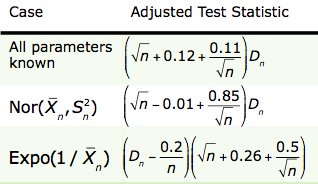
\includegraphics[width=2.5in]{ks01}
\end{figure}
\begin{figure}[!h]
\centering
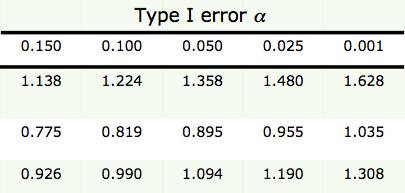
\includegraphics[width=2.5in]{ks02}
\end{figure}
\item Anderson-Darling Test: 
\item No Data: 
\begin{inparaenum}
  \item interview ``experts''; 
  \item Distribution Viewer in ExpertFit; 
  \item interarrival / EXPO; 
  \item \# of ``random'' events in an interval / POIS;
  \item sum of independent ``pieces'' / NORM; 
  \item bounded task times / BETA; and 
  \item unbounded task times / LOGNORMAL or WEIBULL. 
\end{inparaenum}
\end{itemize}

\section*{Output Analysis}
\begin{itemize}
\item Covariance Function: $R_k \equiv \text{Cov}(Y_1,Y_{1+k})$
\[ \text{Var}(\bar{Y}_n) = \frac{1}{n}\left[R_0+2\sum_{k=1}^{n-1}\left(1-\frac{k}{n}\right)R_k\right] \]
\item Types of Simulations: \textbf{Finite-Horizon}, terminate at a specific time or event; \textbf{Steady-State}, long-run behaviour of a system
\item Finite-Horizon: 
\[ S_Z^2 \equiv \frac{1}{b-1}\sum_{i=1}^b(Z_i-\bar{Z}_b)^2 \]
If \# of observations per replication, $m$, is large:
\[ S_Z^2 \approx \frac{\text{Var}(Z_i)\chi^2(b-1)}{b-1}, \theta\in \bar{Z}_b \pm t_{\alpha/2,b-1}\sqrt{S_Z^2/b} \]
\item How to detect initialization bias: attempt to detect the bias visually; or conduct statistical tests. 
\item How to deal with: truncate the output by allowing ``warm up''; or make a very long run to overwhelm the effects of initialization bias. 
\item Steady-State Analysis: 
\[ \sigma^2 = \lim_{n\to\infty}n\text{Var}(\bar{Y}_n) = \sum_{k=-\infty}^{\infty}R_k \]
In \texttt{MA(1)} process, $\sigma^2=(1+\theta)^2$, and \\
In \texttt{AR(1)} process, $\sigma^2=(1+\phi)/(1-\phi)$
\item Batch Means (divided $n=bm$ into $b$ groups): 
\[ \hat{V}_B \equiv \frac{m}{b-1}\sum_{i=1}^b(\bar{Y}_{i,m}-\bar{Y}_n)^2 \approx \frac{\sigma^2\chi^2(b-1)}{b-1} \]
\[ \mu \in \bar{Y}_n \pm t_{\alpha/2,b-1}\sqrt{\hat{V}_B/n} \]
taking $b \approx 30$ and concentrating on increasing the batch size m as much as possible. \\
But problems can come up if the $Y_j$’s are not stationary, if the batch means are not normal, or if the batch means are not independent.
\item Overlapping BM (for large $m$ and $n/m$): 
\[ \bar{Y}_{i,m}^O = \frac{1}{m}\sum_{j=i}^{i+m-1}Y_j,\ \forall i=1,\dots,n-m+1 \]
\[ \hat{V}_O = \frac{m}{n-m+1}\sum_{i=1}^{n-m+1}(\bar{Y}_{i,m}^O-\bar{Y}_n)^2 \]
\[ \mu \in \bar{Y}_n \pm t_{\alpha/2, \frac{3}{2}(b-1)}\sqrt{\hat{V}_O/n} \]
\item Other Methods: Spectral Estimation; Regeneration; Standardized Time Series. 
\item Classical Confidence Intervals: 
\[ \bar{Z}_{i,b_i} \equiv \frac{1}{b_i}\sum\limits_{j=1}^{b_i}Z_{i,j},\ i=1,2 \]
\[ S_i^2 \equiv \frac{1}{b_i-1}\sum\limits_{j=1}^{b_i}(Z_{i,j}-\bar{Z}_{i,b_i})^2,\ i=1,2 \]
\[ \mu_1-\mu_2 \in \bar{Z}_{1,b_1} - \bar{Z}_{2, b_2} \pm t_{\alpha/2,\nu}\sqrt{\frac{S_1^2}{b_1}+\frac{S_2^2}{b_2}} \]
\item Common Random Numbers: the same PRNs
\item Antithetic Variates: negative related PRNs
\item Ranking and Selection Procedures: 
\end{itemize}

\section*{Arena}
\begin{itemize}
\item \emph{Event-Scheduling Approach}: Concentrate on the events and how they affect the system state
\item \emph{Process-Interaction Approach}: Concentrate on a generic customer (entity) and the sequence of events and activities it undergoes as it progresses through the system
\item \emph{Future Events List} (FEL): list of all activities’ scheduled times of completion in chronological order
\item Simulated Time: \texttt{TNOW} \\
Number in Queue: \texttt{NQ(Process.Queue)} \\
\texttt{Name.}: \texttt{NumberIn}, \texttt{NumberOut}, \texttt{WIP}, \texttt{WaitTime}
\item Discrete Probaility: \texttt{DISC}(CumulativeP, V) \\ \texttt{CONT(P,V)}, \texttt{POIS($\lambda$)}, \texttt{EXPO($\lambda$)}, \texttt{NORM($\mu,\sigma$)}, \\ \texttt{TRIA(a,b,c)}, \texttt{UNIF(a,b)}, \texttt{WEIB($\beta,\alpha$)}
\item \textbf{Basic Process}: Create, Process, Decide, Dispose, Assign, Record, Batch, Separate 
\item \textbf{Advanced Process}: Delay, Dropoff, Hold, Match, Pickup, ReadWrite, Release, Remove, Seize, Search, Signal, Store, Unstore, Adjust Variable 
\item \textbf{Advanced Transfer}: Enter, Leave, PickStation, Route, Station, Access, Convet, Exit, Start, Stop, Activate, Allocate, Free, Halt, Move, Request, Transport 
\end{itemize}

\end{document}